
\documentclass[11pt]{article}
\usepackage{amsmath, amssymb}
\usepackage{geometry}
\usepackage{hyperref}
\usepackage{graphicx}
\usepackage{booktabs}
\geometry{margin=2.5cm}

\newcommand{\ket}[1]{|#1\rangle}
\newcommand{\bra}[1]{\langle#1|}
\newcommand{\Oedge}{X_0 Z_1\cdots Z_{L-2} X_{L-1}}

\title{Week 7 Notes: From ED Validation to a Real VQE Sweep}
\author{Seminar notes}
\date{\today}

\begin{document}
\maketitle

\section{Purpose of Week 7}

Week 6 produced an ideal phase diagnostic: a non-local edge string swept across $\mu$ whose magnitude tracks the known topological interval $|\mu|<2t$. That curve was trustworthy, but every plotted point was prepared by exact diagonalization (ED), not by a quantum circuit. The state on which the observable was measured was obtained by diagonalizing the $2^L\times 2^L$ Hamiltonian and reading off the lowest even-parity eigenvector.

Week 7 closes that gap. The milestone is:
\begin{quote}
  Replace the exact-diagonalization state preparation with a parity-constrained VQE preparation at every point of the $\mu$ sweep, and validate each prepared state against ED before any hardware noise is introduced.
\end{quote}

Everything else from Week 6 is kept fixed: the same Hamiltonian, the same edge-string observable $O_{\mathrm{edge}}=\Oedge$, the same shot-measurement protocol, and the same $\mu$ grid. The only change is how the state is produced. This isolates a single question: can a variational quantum circuit reproduce the ideal diagnostic curve well enough to serve as the noiseless baseline for the Block 4 noise study?

\section{What Changes Conceptually from Week 6}

Week 6 answered ``does the chosen observable reconstruct the phase diagram?'' using a trusted ED reference state. Week 7 answers a different, harder question:
\begin{quote}
  ``Can a gate-based, variationally optimized state reproduce that diagnostic across the whole parameter range?''
\end{quote}

This is the step from a numerically exact target to an algorithm that must actually find the ground state. Three new difficulties appear that ED never had to confront:
\begin{enumerate}
  \item the optimizer can fail or land in a local minimum;
  \item the optimizer can drift into the wrong fermion-parity sector;
  \item near criticality the ground state changes fastest, so a single ansatz must remain expressive enough everywhere.
\end{enumerate}
Week 7 is largely about controlling these three failure modes and proving, point by point, that they did not occur.

\section{Hamiltonian and Observable (Unchanged)}

The Jordan--Wigner mapping of the open Kitaev chain gives
\begin{equation}
  H(\mu)
  = -\frac{\mu}{2}\sum_{j=0}^{L-1} Z_j
    + \frac{t-\Delta}{2}\sum_{j=0}^{L-2} X_jX_{j+1}
    + \frac{t+\Delta}{2}\sum_{j=0}^{L-2} Y_jY_{j+1}.
\end{equation}
As in Week 6 we use $L=4$ and the sweet-spot couplings
\begin{equation}
  t=\Delta=1,
\end{equation}
so the $XX$ term vanishes and
\begin{equation}
  H(\mu) = -\frac{\mu}{2}\sum_j Z_j + \sum_{j=0}^{L-2} Y_jY_{j+1},
  \qquad \mu_c = \pm 2t.
\end{equation}
The plotted quantity remains the magnitude of the parity-preserving edge string
\begin{equation}
  |\langle O_{\mathrm{edge}}\rangle|, \qquad O_{\mathrm{edge}}=\Oedge,
\end{equation}
which for $L=4$ is $X_0 Z_1 Z_2 X_3$. The motivation for using a non-local string rather than a local edge operator is identical to Week 6: any operator anticommuting with parity has zero expectation value in a parity eigenstate, so only a parity-preserving, non-local observable is a stable diagnostic.

\section{The VQE Sweep Workflow}

The core of Week 7 is a loop over the $\mu$ grid. For each $\mu_k$ the workflow is:
\begin{enumerate}
  \item build the Pauli-term Hamiltonian $H(\mu_k)$;
  \item initialize the variational parameters from the previous point, $\theta_k \leftarrow \theta_{k-1}^{*}$ (warm start);
  \item minimize the parity-constrained cost to obtain $\theta_k^{*}$;
  \item validate the resulting state against the ED reference (energy, parity, subspace fidelity, edge-string error);
  \item if validation fails, recover with random restarts and deeper optimization;
  \item measure $|\langle O_{\mathrm{edge}}\rangle|$ both ideally and with finite shots;
  \item store the parameters, diagnostics, and observable, then advance to $\mu_{k+1}$.
\end{enumerate}

The single most important engineering change relative to Week 6 is that the optimizer is no longer restarted independently at each $\mu$. Neighboring ground states seed one another.

\section{Warm-Start Continuation}

The ground state of $H(\mu)$ evolves smoothly with $\mu$ away from the critical points. Continuation exploits this: the optimal parameters at one point are a good initial guess for the next.

\paragraph{Independent random starts (the Week 5/6 prototype style).}
\begin{itemize}
  \item repeat expensive optimization work at every point;
  \item can converge to different local minima at adjacent $\mu$, producing artificial jumps;
  \item make the swept curve noisy even before shot noise is added.
\end{itemize}

\paragraph{Continuation in $\mu$.}
\begin{itemize}
  \item initialize $\theta_{k+1}$ from $\theta_k^{*}$;
  \item track the smooth evolution of the ground state efficiently;
  \item keep random restarts only as a fallback when validation fails.
\end{itemize}

The expected difficulty is concentrated near $|\mu|=2t$, where the bulk gap closes and the optimal state changes fastest. This is exactly where warm starts and fidelity checks matter most, and where the recovery path is most likely to trigger.

\section{Parity Must Be Controlled}

The Hamiltonian conserves fermion parity,
\begin{equation}
  P=\prod_{j=0}^{L-1}Z_j, \qquad [H,P]=0.
\end{equation}
In the topological phase the even- and odd-parity sectors are nearly degenerate. Plain energy minimization can therefore return different sectors at different $\mu$, and a sector flip looks like a spurious discontinuity in $\langle O_{\mathrm{edge}}\rangle$.

The Week 7 strategy is to bias the optimization toward a fixed (even) sector with a parity penalty:
\begin{equation}
  C(\theta) = \langle H\rangle_\theta + \lambda\bigl(1-\langle P\rangle_\theta\bigr)^2.
\end{equation}
The penalty is minimized when $\langle P\rangle = +1$, pushing the optimizer into the even sector without distorting the energy landscape inside that sector. The parity expectation $\langle P\rangle$ is recorded at every point, and states that fall outside the parity tolerance are rejected and recovered.

\section{Validation Dashboard}

A low VQE energy alone is not a sufficient acceptance criterion near degeneracy. Each swept point must pass four independent checks against the ED reference:

\begin{center}
\begin{tabular}{p{0.20\textwidth}p{0.33\textwidth}p{0.33\textwidth}}
\toprule
\textbf{Metric} & \textbf{Question} & \textbf{Purpose} \\
\midrule
Energy error & Is $E_{\mathrm{VQE}}$ near $E_{\mathrm{ED}}$? & Detect optimizer failure \\
Parity & Is $\langle P\rangle\approx +1$? & Keep one sector across the sweep \\
Subspace fidelity & Does the VQE state overlap the correct low-energy space? & Handle near-degeneracy correctly \\
String error & Does $\langle O_{\mathrm{edge}}\rangle$ match the ED value? & Validate the quantity actually plotted \\
\bottomrule
\end{tabular}
\end{center}

Subspace fidelity (rather than overlap with a single eigenvector) is the right measure because the two lowest states are nearly degenerate in the topological phase; the prepared state only needs to live in that low-energy subspace. A point that fails any check triggers deeper ansatz repetitions, more optimizer iterations, or random-restart recovery.

\section{Implementation Shape}

The loop body, in schematic form, is:
\begin{verbatim}
theta = initial_parameters()
for mu in mu_values:
    H = qiskit_hamiltonian(L, t, mu, delta)
    theta = optimize(parity_cost(H), initial=theta)

    diagnostics = validate(theta, H, ed_reference(mu))
    if not diagnostics.pass_all:
        theta = recover_with_restarts(H)

    string_value = measure_edge_string(theta, shots=4096)
    save(mu, theta, diagnostics, string_value)
\end{verbatim}

\begin{sloppypar}
The implementation lives in \texttt{src/block3\_core.py} (helpers \texttt{vqe\_cost}, \texttt{evaluate\_state}, \texttt{solve\_point}, \texttt{vqe\_sweep}, \texttt{measure\_edge\_string\_shots}, \texttt{best\_state}, \texttt{depth\_scan}) and is driven by \texttt{src/block3.py --plots 7} (the sweep) and \texttt{--plots 8} (the depth diagnostic). The ansatz is the same hardware-efficient \texttt{EfficientSU2} with $R_Y$ rotations and linear CNOT entanglement used in Week 5. A practical point: the sweep must persist optimizer parameters and per-point diagnostics, not only the final observable, so that failed regions are debuggable and reusable as warm starts for later noise studies.
\end{sloppypar}

\section{Reading the Week 7 Sweep Figure}

\begin{figure}[h]
  \centering
  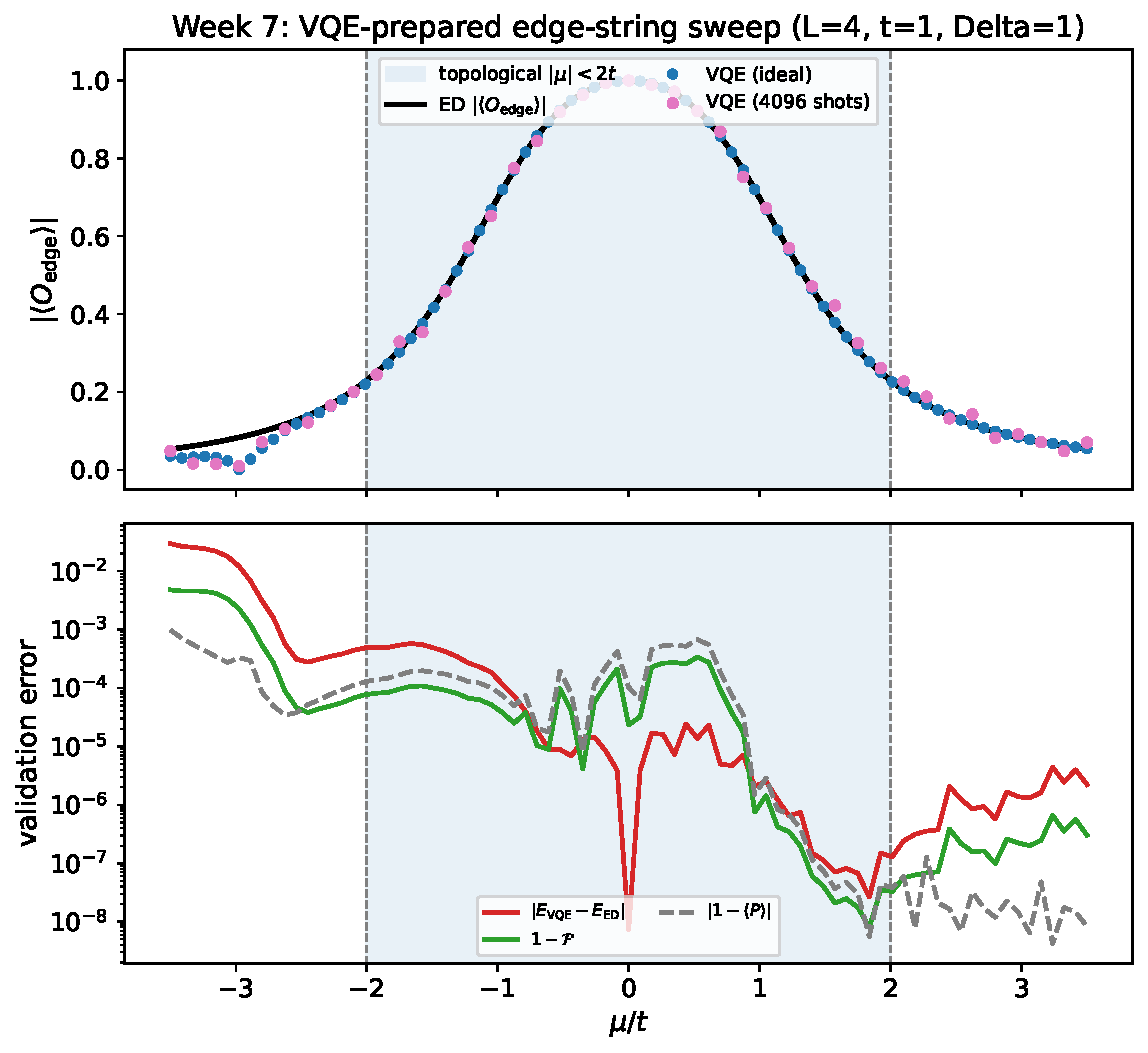
\includegraphics[width=0.9\linewidth]{../plots/block3_week7_vqe_sweep.pdf}
  \caption{Week 7 VQE-prepared sweep for $L=4$, $t=\Delta=1$. Top: the edge string $|\langle O_{\mathrm{edge}}\rangle|$ from parity-constrained VQE, both ideal and shot-based, plotted against the ED baseline. Bottom: per-point validation showing energy error, infidelity $1-\mathcal{F}$, and parity deviation $|1-\langle P\rangle|$; crosses mark points that required random-restart recovery.}
\end{figure}

The expected behavior is:
\begin{itemize}
  \item the VQE curve (ideal and shot-based) overlays the ED baseline across the whole $\mu$ grid;
  \item energy error and infidelity stay near zero inside the topological region and rise mildly near $|\mu|=2t$;
  \item parity deviation stays small everywhere because the penalty pins the even sector;
  \item recovery markers, if any, cluster near criticality where the optimization is hardest.
\end{itemize}
The top panel is the measurement-side result that Block 4 will compare against; the bottom panel is the certificate that the result was obtained from genuinely correct state preparation.

\section{Ansatz Depth: How Deep Is Enough?}

\begin{figure}[h]
  \centering
  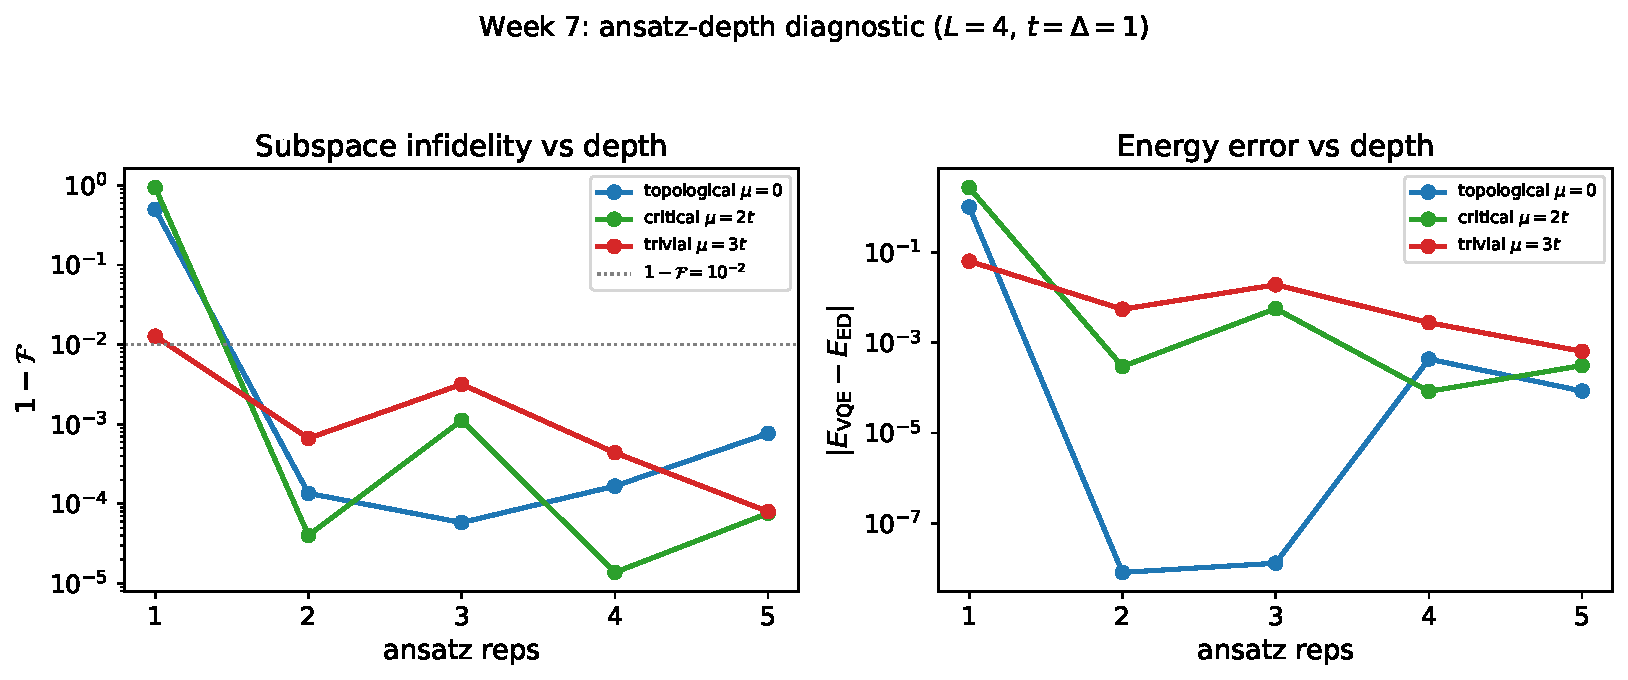
\includegraphics[width=0.85\linewidth]{../plots/block3_week7_depth_fidelity.pdf}
  \caption{Ansatz-depth diagnostic: multi-start VQE subspace infidelity and energy error versus the number of ansatz repetitions, at three representative $\mu$ (topological, critical, trivial).}
\end{figure}

Scanning the number of \texttt{EfficientSU2} repetitions establishes the minimum depth needed for faithful preparation:
\begin{itemize}
  \item one repetition ($8$ parameters) is too shallow; it fails worst at criticality $\mu=2t$ (fidelity $\sim 0.06$);
  \item two or more repetitions already reach the even-parity ground space;
  \item the critical point is consistently the hardest, exactly where the bulk gap closes.
\end{itemize}
This justifies the choice \texttt{reps}$=3$ used in the full sweep: deep enough to clear criticality with margin, shallow enough to keep the optimization cheap.

\section{Definition of Done for Week 7}

\begin{itemize}
  \item a scripted $L=4$, $t=\Delta=1$ VQE sweep over the same $\mu$ grid as Week 6;
  \item consistent even-parity preparation across the entire sweep;
  \item ED comparison for energy, parity, subspace fidelity, and edge-string expectation at every point;
  \item a shot-based VQE edge-string curve plotted against the ED baseline;
  \item optimization cost and failure/recovery statistics recorded per $\mu$ point.
\end{itemize}

\section{Bridge to Block 4}

Week 7 validates quantum state preparation; it does not yet test robustness. Only after the ideal VQE sweep passes validation should noise be introduced. The Block 4 plan is:
\begin{itemize}
  \item freeze the validated ideal VQE sweep as the noiseless reference;
  \item apply realistic gate, readout, and relaxation ($T_1$, $T_2$) noise to the preparation and measurement circuits;
  \item separate optimizer degradation from measurement degradation;
  \item compare raw and error-mitigated edge-string curves;
  \item quantify the noise level at which the inferred phase boundary becomes unreliable.
\end{itemize}

The conceptual progression across the block is now complete in outline: Week 6 validated the diagnostic with ED, Week 7 validates the quantum state preparation, and Block 4 tests whether the full circuit workflow survives realistic noise.

\end{document}
